\chapter{Das Lösungskonzept}
\label{cha:Lösungskonzept}
In diesem Kapitel wird der Lösungsansatz und die Spezifikation des Vorlagenmanagements behandelt. Bei der Spezifikation handelt es sich um die Schnittstellen und die abstrakte Klassen, die die Struktur des Vorlagenmanagements definieren und gemeinsame Logik vorgegeben. Diese Schnittstellen und abstrakten Klassen erlauben es Implementierungen für verschiedene \emph{Template-Engines} zur Verfügung zu stellen wie z.B.
\begin{itemize}
	\item für die \emph{Template-Engine Freemakrer},
	\item für die \emph{Template-Engine Velocity} oder
	\item für die \emph{Template-Engine Thymeleaf}.
\end{itemize}
\ \newline
Mit der Möglichkeit verschiedene \emph{Template-Engines} verwenden zu können, soll das Vorlagenmanagement flexible gehalten werden. Bei einem Wechsel zu einer anderen \emph{Template-Engine}, müssen nur die Ausdrücke in einer Vorlagen in die \emph{Template-Engine} spezifischen Ausdrücke konvertiert werden, was sich einfach realisieren lässt, da die Ausdrücke einer Vorlage immer gefunden werden müssen.

\section{Die Spezifikation des Vorlagenmanagements}
\label{sec:specification-template-management}
Dieses Kapitel behandelt die erstellten Spezifikationen des Vorlagenmanagements. Auf Basis dieser Spezifikationen wird das Vorlagenmanagement und die Integrationen in die verschiedenen Umgebungen und Technologien implementiert. Die erstellte Spezifikationen sind frei von Abhängigkeiten auf konkrete Implementierungen jeglicher Art. Sie haben nur Abhängigkeiten auf andere Spezifikationen wie die \emph{JEE-7} Spezifikation.
\newpage

\begin{figure}[h]
\centering
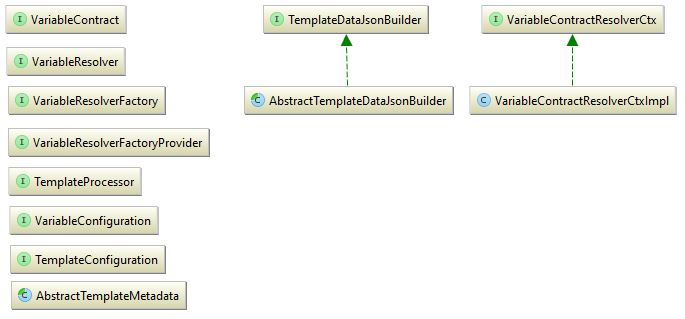
\includegraphics[scale=0.73]{20160710_template-logic-api.jpg} %{CS0031}
\caption{Klassenhierarchie des Vorlagenmanagements}
\label{fig:template-logic-api-hierarchy}
\end{figure}

\subsection{Die Schnittstellen und abstrakten Klassen}
Dieser Abschnitt behandelt die definierten Schnittstellen und abstrakten Klassen des Vorlagenmanagements. Die abstrakten Klassen implementieren die gemeinsame nutzbare Logik, die von alle konkreten Implementierungen des Vorlagenmanagements für jede \emph{Template-Engine} genutzt werden können. Diese Spezifikationen spezifizieren Aspekte des Vorlagenmanagements wie
\begin{enumerate}
	\item das Variablenmanagement innerhalb des Vorlagenmanagement,
	\item die Handhabung von Variablen in einer Vorlage,
	\item die Abbildung der Metadaten einer Voralge und 
	\item das Erstellen des \emph{JSON}-Datenobjekts, welches die serialisierten Daten der Variablen einer Vorlage, sowie Metadaten enthält.
\end{enumerate}

\subsubsection{Die Schnittstelle \emph{VariableContract}}
\label{sec:variableContract}
Die Schnittstelle \emph{VariableContract} aus Abbildung \ref{prog:variableContract} spezifiziert eine Variable, die in einer Vorlage verwendet werden kann. Objekte dieser Schnittstelle werden beim Anwendungsstart registriert und können grundsätzlich in allen Vorlagen verwendet werden. Eine Variable ist einem Modul zugeordnet, in dem die Variable bezüglich ihres Namen eindeutig sein muss. Das Modul wird über eine Zeichenkette definiert. Die Mehrsprachigkeit einer Variable wird über Enumerationen realisiert, wobei jede Variable jeweils einen Schlüssel für den Titel und die Beschreibung bereit stellen muss.
\newline
\newline
Da es sich bei einer Variable um statische Daten handelt, also die Variablen sind schon zur Kompilierungszeit bekannt, ist angedacht, dass die Variablen als Enum implementiert werden, das die Schnittstelle \emph{VariableContract} implementiert. Durch die Abbildung der Variablen mit einer Enum können mehrere Variablen in einer Klasse definiert werden, wobei eine einzelne Enumeration der Enum ein Objekt der Schnittstelle \emph{VariableContract} darstellt. Alle Variablen, die mit einer Enum abgebildet werden, sollten demselben Modul zugeordnet sein, obwohl dies nicht zwingend erforderlich ist. Die Zuordnung der Variablen zum selben Modul erleichtert die Organisation der Variablen. Die Variablen, die mit einer Enum definiert wurden, werden innerhalb des Vorlagenmanagements trotzdem als einzelne Objekte der Schnittstelle \emph{VariableContract} betrachtet. Die Tatsache dass die Variablen mit einer Enum abgebildet wurden, ist für das Vorlagenmanagement nur beim Registrieren der Variablen von belang und nicht bei deren weiterer Verwendung.
\newline
\newline
Eine Variable ist über seine \emph{Id} global eindeutig identifizierbar, wobei sich die \emph{Id} aus dem Modulnamen und den Variablennamen zusammensetzt (Bsp. module.core.VAR\_1). Die \emph{Id} sowie der Modulname muss sich dabei an die Namenskonvention eines \emph{Java}-Paketnamen halten. Da der Variablenname immer auf diese Weise zusammengesetzt werden muss, wurde die Methode \emph{String getId();} als \emph{Default Methode} implementiert, was seit \emph{Java 8} möglich ist. Ein EntwicklerIn muss diese Methode nicht mehr implementieren, obwohl es immer noch möglich ist diese Methode zu überschreiben. Auch die Methode \emph{String toInfoString()} wurde als \emph{Default Methode} implementiert, da auch diese Methode nicht von den EntwicklerInnen implementiert werden sollte, da ihre Funktionalität sich nicht ändern sollte.
\newpage

\begin{program}[h]
\caption{Die Schnittstelle \emph{VariableContract}}
\label{prog:variableContract}
\begin{JavaCode}
public interface VariableContract extends Serializable {

    String getName();

    String getModule();

    Enum<?> getInfoKey();

    Enum<?> getLabelKey();

    default String getId() {      
        return getModule() + "." + getName();
    }

    default String toInfoString() {
        final String ls = System.lineSeparator();
        final StringBuilder sb = new StringBuilder();
        sb.append("contract  : ").append(this.getClass().getName())
          .append(ls)
          .append("id        : ").append(getId())
          .append(ls)
          .append("name      : ").append(getName())
          .append(ls)
          .append("label-key : ").append((getLabelKey() != null) 
                                          ? getLabelKey().name() 
                                          : "not available")
          .append(ls)
          .append("info-key  : ").append((getInfoKey() != null) 
                                          ? getInfoKey().name() 
                                          : "not available")
          .append(ls)
          .toString();
    }
}
\end{JavaCode}
\end{program}

\subsubsection{Die Schnittstelle \emph{VariableResolver}}
\label{sec:variableResolver}
Die Schnittstelle \emph{VariableResolver} aus Abbildung \ref{prog:variableResolver} spezifiziert wie der aktuelle Wert der Variablen aufgelöst wird. Eine Variable wird in einer Vorlage verwendet und beim Erstellen einer \emph{E-Mail}, die diese Vorlage verwendet, müssen die aktuellen Werte der beinhalteten Variablen aufgelöst werden. Da der aktuelle Wert der Variable kontextabhängig ist, wird beim Auflösen des Werts der Variable ein Kontextobjekt bereitgestellt, über den kontextabhängige Daten von den  EntwicklerInnen bereitgestellt werden können. Durch dieses Kontextobjekt kann die Variable in mehreren Kontexten verwendet werden und auch kontextabhängig aufgelöst werden.
\begin{program}[h]
\caption{Die Schnittstelle \emph{VariableResolver}}
\label{prog:variableResolver}
\begin{JavaCode}
@FunctionalInterface
public interface VariableResolver {

    String resolve(VariableContract variable,
                   VariableContractResolverContext ctx);
}
\end{JavaCode}
\end{program}
\ \newline
Die Schnittstelle \emph{VariableResolver} wurde als \emph{FunctionalInterface} implementiert. Ein \emph{FunctionalInterface} ist eine Schnittstelle, die nur eine abstrakte Methode definiert, die implementiert werden muss. Eine Implementierung eines \emph{FunctionalInterface} kann über eine \emph{Lambda}-Funktion oder Methodenreferenz bereitgestellt werden, wodurch die Notwendigkeit einer anonymen Implementierung oder der Implementierung einer Klasse für diese Schnittstelle entfällt. Die Verwendung von \emph{Lambda}-Funktionen und Methodenreferenzen macht den Quelltext lesbarer, obwohl angemerkt sei, dass dieser Ansatz sich negativ auf das Laufzeitverhalten auswirkt, was in der Art und Weise der Ausführung einer \emph{Lambda}-Funktion oder Methodenreferenz begründet ist. Die negativen Auswirkungen auf das Laufzeitverhalten können, im Bezug auf das Vorlagenmanagement, vernachlässigt werden.

\subsubsection{Die Schnittstelle \emph{VariableResolverFactory}}
\label{sec:variableResolverFactory}
Die Schnittstelle \emph{VariableResolverFactory} aus Abbildung \ref{prog:variableResolverFactory}  spezifiziert wie Objekte der Schnittstelle \emph{VariableResolver} produziert werden. Objekte dieser Schnittstelle können Objekte der Schnittstelle \emph{VariableResolver} für jede Implementierung der Schnittstelle \emph{VariableContract} produzieren. Es wird aber empfohlen, dass es je eine Implementierung der Schnittstelle \emph{VariableResolverFactory} je Modul gibt.

\begin{program}[h]
\caption{Die Schnittstelle \emph{VariableResolverFactory}}
\label{prog:variableResolverFactory}
\begin{JavaCode}
@FunctionalInterface
public interface VariableResolverFactory extends Serializable {

  VariableResolver getVariableResolver(VariableContract contract,
                                       VariableContractResolverCtx ctx);
}
\end{JavaCode}
\end{program}
\ \newline
Die Schnittstelle \emph{VariableResolver} wurde auch als \emph{FunctionalInterface} implementiert, damit Implementierungen über eine \emph{Lambda}-Funktion oder eine Methodenreferenz bereitgestellt werden kann.

\subsubsection{Die Schnittstelle \emph{VariableResolverFactoryProvider}}
\label{sec:VariableResolverFactoryProvider}
Die Schnittstelle \emph{VariableContractFactoryProvider} aus Abbildung \ref{prog:variableResolverFactoryProvider} spezifiziert wie Objekte der Schnittstelle \emph{VariableResolverFacotry} produziert werden. Ein Objekt der Schnittstelle \emph{VariableResolverFactoryProvider} kann Objekte der Schnittstelle \emph{VariableResolverFactory} für die Schnittstelle \emph{VariableContract}, einer Ableitung von dieser Schnittstelle oder einer konkreten Implementierung dieser Schnittstelle zur Verfügung stellen. Die Schnittstelle \emph{VaraibleResolverFactoryProvider} wurde spezifiziert, damit in einer \emph{CDI}-Umgebung über ein Objekt dieser Schnittstelle die Objekte der Schnittstelle \emph{VariableResolverFactory} produziert werden können, die von der \emph{CDI}-Umgebung zur Verfügung gestellt werden.

\begin{program}[h]
\caption{Die Schnittstelle \emph{VariableResolverFactoryProvider}}
\label{prog:variableResolverFactoryProvider}
\begin{JavaCode}
@FunctionalInterface
public interface VariableResolverFactoryProvider extends Serializable {

    VariableResolverFactory getVariableResolverFactory
            (Class<? extends VariableContract> contractType);
}
\end{JavaCode}
\end{program}
\ \newline
Die Schnittstelle \emph{VariableResolverFactoryProvider} wurde auch als \emph{FunctionalInterface} implementiert, damit Implementierungen über eine \emph{Lambda}-Funktion oder eine Methodenreferenz bereitgestellt werden kann.

\subsubsection{Die Schnittstelle \emph{VariableContractResolverCtx}}
\label{sec:variableResolverFactoryProvider}
Die Schnittstelle \emph{VariableContractResolverCtx} aus Abbildung \ref{prog:variableContractResolverCtx} spezifiziert den Kontext, der bei der beim Auflösen des aktuellen Werts der Variablen zur Verfügung gestellt wird. Dieser Kontext stellt alle Daten bereit, die beim Auflösen des aktuellen Werts einer Variable benötigt werden. Es wird auch ermöglicht, dass Benutzerdaten im Kontext definiert werden können, die bei beim Auflösen des aktuellen Werts einer Variable verwendet werden können. Es wurde bewusst vermieden, dass beim Auflösen eines aktuellen Werts einer Variable bekannt ist, in welcher Vorlage die Variable verwendet wird. Dadurch bleibt die Handhabung der Variablen einer Vorlage entkoppelt von der Vorlage selbst. Dadurch wäre es möglich die Variablen außerhalb vom Vorlagenmanagements zu verwenden.
\newpage

\begin{program}[h]
\caption{Die Schnittstelle \emph{VariableContractResolverCtx}}
\label{prog:variableContractResolverCtx}
\begin{JavaCode}
public interface VariableContractResolverCtx {

    Locale getLocale();

    ZoneId getZoneId();

    TimeZone getTimeZone();

    <T> T getUserData(Object key,
                      Class<T> clazz);
}
\end{JavaCode}
\end{program}

\subsubsection{Die Schnittstelle \emph{TemplateProcessor}}
\label{sec:templateProcessor}
Die Schnittstelle \emph{TemplateProcessor} aus Abbildung \ref{prog:templateProcessor} spezifiziert wie die Variablen in einer Vorlagen behandelt werden. Objekte dieser Schnittstelle können Variablen in einer Vorlage, einer bestimmten \emph{Template-Engine} finden und konvertieren. Ein \emph{TemplateProcessor} muss ebenfalls in der Lage sein ungültige Variablen innerhalb einer Vorlage zu finden, wobei eine ungültige Variable eine Variable ist, die nicht registriert ist und somit die variable nicht bekannt ist. Eine konkrete Implementierung der Schnittstelle \emph{TemplateProcessor} ist eine Implementierung für eine bestimmte \emph{Template-Engine}, da die in der Vorlage verwendeten Variablen in Form von Ausdrücken spezifisch für die verwendete \emph{Template-Engine} sind. 
\newline
\newline
Der Quelltext aus Abbildung \ref{prog:templateProcessor-highlighted-methods} zeigt die beiden Konvertierungsmethoden der Schnittstelle \emph{TemplateProcessor}.
\begin{program}[h]
\caption{Die Methoden für die Konvertierung}
\label{prog:templateProcessor-highlighted-methods}
\begin{JavaCode}[numbers=none]
String replaceExpressions(String template,
                          Function<VariableContract, String> converter);

String replaceCustom(String template,
                     Pattern itemPattern,
                     Function<String, String> converter);
\end{JavaCode}
\end{program}
\ \newline
Diese Methoden definieren als Formalparameter für den benötigte Konverter ein \emph{FunctionalInterface} namens \emph{Function}, welches von \emph{Java 8} bereitgestellt wird. Dadurch ist das Spezifizieren einer eigenen Schnittstelle für die Konvertierung nicht mehr nötig. Der Konverter kann über eine \emph{Lambda}-Funktion oder Methodenreferenz bereitgestellt werden. Dadurch ist die Konvertierung der Variablen einer Vorlage abstrahiert von der Implementierung der Schnittstelle \emph{TemplateProcessor}, wodurch die Variablen durch eine beliebige Repräsentation ersetzt werden können und visa versa.

\begin{program}[h]
\caption{TemplateProcessor.java}
\label{prog:templateProcessor}
\begin{JavaCode}
public interface TemplateProcessor {

    String replaceExpressions(String template,
                              Function<VariableContract, String> converter);

    String replaceCustom(String template,
                         Pattern itemPattern,
                         Function<String, String> converter);

    Set<VariableContract> resolveExpressions(String template);

    Set<String> resolveInvalidExpressions(String template);

    String variableToExpression(VariableContract contract);

    VariableContract expressionToVariable(String expression);
}
\end{JavaCode}
\end{program}

\subsubsection{Die Schnittstelle \emph{TemplateDataJsonBuilder}}
\label{sec:templateDataJsonBuilder}
Die Schnittstelle \emph{TemplateDataJsonBuilder} aus Abbildung \ref{prog:templateDataJsonBuilder} spezifiziert die Signatur eines \emph{Builders}, der das Datenobjekt erstellt, welches die Daten für das Parsen einer Vorlage enthält. Die \emph{E-Mail}-Nachrichten werden persistent zu halten, wobei nach der Erstellung einer \emph{E-Mail}-Nachricht, dessen Inhalt unveränderbar sein muss. Das Datenobjekt enthält die folgenden Daten wie
\begin{itemize}
	\item die Sprache in der die \emph{E-Mail} versendet wird,
	\item die Zone für die Konvertierung von Datums- und Zeitwerten,
	\item die Version der Vorlage und 
	\item die Metadaten der Vorlage wie z.B die Anzahl der enthaltenen Variablen.
\end{itemize} 
Dieses Datenobjekt kann als \emph{JSON} in den folgenden Formen vom \emph{Builder} bereitgestellt werden.
\begin{itemize}
	\item Als \emph{Java}-Objekt,
	\item als \emph{JSON}-Zeichenkette und
	\item als Objekt der Klasse \emph{java.util.Map}.
\end{itemize}
\ \newline
Anstatt der Serialisierung der Daten könnte auch die Vorlage geparst werden und die gesamte Vorlage persistent gehalten werden, wodurch aber die Menge an persistent gehaltenen Daten stark ansteigen würde. Mit einem Datenobjekt werden nur die benötigten Daten persistent gehalten, wodurch die Menge an persistent gehaltenen Daten so klein wie möglich gehalten wird. Mit diesem Datenobjekt kann die korrespondierende Vorlage zu jedem Zeitpunkt mit demselben Resultat wiederhergestellt werden.
\newline
\newline
Es wurde hier das \emph{Builder}-Muster angewendet, da sich die Konfiguration des \emph{Builders} mit einer \emph{Fluent-API}, wie bei einem \emph{Builder} üblich, sehr gut abbilden lässt. Die Schnittstelle \emph{TemplateDataJsonBuilder} spezifiziert folgende Terminalmethoden.
\begin{itemize}
	\item\emph{TemplateRequestJson toJsonModel();}
	\newline
	ist die Methode, die das Datenobjekt in Form eines \emph{Java}-Objekts zurückliefert.
	\item\emph{String toJsonString();}
	\newline
	ist die Methode, die das Datenobjekt als Zeichenkette zurückliefert.
	\item\emph{Map<String, Object> toJsonMap();}
	\newline
	ist die Methode, die das Datenobjekt in Form eines Objekts der Klasse \emph{java.util.Map} zurückliefert.
\end{itemize} 
\ \newline 
Der Quelltext aus Abbildung \ref{prog:templateDataJsonBuilder-example} illustriert, wie der \emph{Builder} verwendet wird.
\begin{program}[h]
\caption{Beispiel einer Anwendung des \emph{Builders}}
\label{prog:templateDataJsonBuilder-example}
\begin{JavaCode}
builder.withStrictMode() 
       .withLocalization(localeObj, zoneIdObj)
       .withTemplate(templateMetadataObj)
       .withUserData(userDataMap)
       .withVariableResolverFactoryProvider(factoryProviderObj)
       .toJsonModel();
\end{JavaCode}
\end{program}

\begin{program}[h]
\caption{TemplateDataJsonBuilder.java}
\label{prog:templateDataJsonBuilder}
\begin{JavaCode}
public interface TemplateDataJsonBuilder<I,
    M extends AbstractTemplateMetadata<I>,
    B extends TemplateDataJsonBuilder> extends Serializable {

    B withWeakMode();

    B withLocalization(Locale locale,
                       ZoneId zoneId);

    B withUserData(Map<Object, Object> userData);

    B withStrictMode();

    B withVariableResolverFactoryProvider
                         (VariableResolverFactoryProvider factory);

    B withVariableResolverFactory(VariableResolverFactory factory);

    B withTemplate(M metadata);

    void end();

    B addVariable(VariableContract contract,
                  Object value);

    B addVariableResolver(VariableContract contract,
                          VariableResolver resolver);

    TemplateRequestJson toJsonModel();

    String toJsonString();

    Map<String, Object> toJsonMap();
}
\end{JavaCode}
\end{program}
\ \newpage

\subsubsection{Die abstrakte Klasse \emph{AbstractTemplateMetadata}}
\label{sec:abstractTemplateMetadata}
Die abstrakte Klasse \emph{AbstractTemplateMetadata} implementiert die Logik, die von allen konkreten Implementierungen dieser abstrakten Klasse für die verschiedenen \emph{Template-Engines} genutzt werden kann. Die Metadaten wie
\begin{itemize}
	\item die Anzahl der gültigen Variablen in der Vorlage,
	\item die Anzahl der ungültigen Variablen in der Vorlage,
	\item die Zeichenlänge der Vorlage,
	\item die eindeutige \emph{Id} der Vorlage,
	\item die Version der Vorlage und
	\item die Vorlage selbst
\end{itemize}
werden in dieser Klasse abgebildet. Diese Metadaten sind unabhängig der verwendeten \emph{Template-Engine} und eine konkrete Implementierung für eine \emph{Template-Engine} kann zusätzliche Metadaten definieren. Die Metadaten werden einmalig ermittelt und sind über die Lebenszeit des Objekts unveränderbar. Wird die Vorlage geändert so muss auch eine neues Objekt der Metadaten erstellt werden.
\newline
\newline
\emph{TODO: Add source as appendix, because to long ?}

\subsubsection{Die abstrakte Klasse \emph{AbstractTemplateDataJsonBuilder}}
\label{sec:abstractTemplateDataJsonBuilder}
Die abstrakte Klasse \emph{AbstractTemplateDataJsonBuilder} implementiert die gemeinsam nutzbare Logik, die von allen konkreten Implementierungen für die verschiedenen \emph{Template-Engines} verwendet werden kann. Sie stellt Hilfsmethoden bereit, die Variablen innerhalb der Vorlage finden, validieren und deren aktuellen Wert auflösen können. Das resultierende Datenobjekt des \emph{Builders} ist spezifiziert, jedoch nicht die Abbildung der aufgelösten Werte für die enthaltenen Variablen. Diese Daten sind spezifisch für die verwendete \emph{Template-Engine}.
\newline 
\newline  
\emph{TODO: Add source as appendix, because to long ?}

\section{Die Spezifikation der Vorlagenintegration}
Die im Abschnitt \ref{sec:specification-template-management} vorgestellte Spezifikation des Vorlagenmanagements, spezifiziert die Kernfunktionalität des Vorlagenmanagements, dass in der Lage ist die Vorlagen sowie deren enthaltene Variablen zu behandeln. Das Vorlagenmanagement benötigt auch Integrationen in verschiedene Umgebungen und Sprachen, um die benötigte Funktionalitäten wie
\begin{itemize}
	\item die Verwaltung der Variablen in einem \emph{Javascript} basierten \emph{CKEditor},
	\item die automatische Registrierung der Variablen in einer \emph{CDI}-Umgebung,
	\item die Verwaltung der Vorlagen in einer Webseite und
	\item die Persistenz der Vorlagen realisieren zu können. 
\end{itemize}
Folgender Abschnitt behandelt die Spezifikationen der Integrationen wie in Abschnitt \ref{sec:technical-goals} vorgegeben. 
 
\subsection{Das Vorlagenmanagement in \emph{Typescript}}
\label{sec:sub-typescript-javascript}
Es muss der \emph{Rich-Editor CKEditor} verwendet werden, mit dem \emph{HTML} basierte Vorlagen in einer Webseite verwaltet werden können. Der \emph{CKEditor} muss angepasst werden, damit die definierten Variablen in einer Vorlage verwendet werden können. Wie in Abschnitt \ref{sec:sub-template-management-website} vorgegeben, wird der \emph{CKEDitor} verwendet, für den es bereits eine Integration in \emph{JSF} in Form einer \emph{JSF}-Komponente gibt, die von \emph{primefaces-extensions} zur Verfügung gestellt wird. Es wird ein \emph{CKEditor-Plugin} in \emph{Typescript} entwickelt, das es erlaubt, die definierten Variablen innerhalb des \emph{CKEditors} und dessen enthaltener Vorlage zu verwalten. Es wird die Skriptsprache \emph{Typescript} verwendet, da es mit dieser Skriptsprache möglich ist typsicher zu entwickeln, was in \emph{Javascript} nicht möglich ist. Ebenfalls kann \emph{Typescript} in mehrere \emph{ECMA}-Standards übersetzt werden.
\newline
\newline
Innerhalb des \emph{CKEditor-Plguins} werden Variablen verwendet, dessen Management in einer eigenen Quelltextdatei implementiert wird, da es unabhängig von \emph{CKEditor-Plguin} ist und daher auch anderweitig verwendet werden kann. Damit wird das Variablenmanagement entkoppelt vom \emph{CKEditor-Plugin}.

\subsection{Das Vorlagenmanagement in \emph{CDI}}
\label{sec:sub-template-management-cdi}
Das Vorlagenmanagement wird in einem \emph{JEE-7}-Anwendungsserver verwendet, der eine \emph{CDI}-Umgebung bereitstellt. Im \emph{CDI}-Standard sind portable Erweiterungen  spezifiziert, die es erlauben, dass sich Softwarekomponenten in einer \emph{CDI}-Umgebung integrieren. Es wird eine \emph{CDI}-Erweiterung implementiert, die beim Start der \emph{CDI}-Erweiterung, die definierten Variablen automatisch registriert und über den Lebenszyklus der Anwendung persistent hält. Es sollen Ressourcen des Vorlagenmanagements wie z.B
\begin{itemize}
	\item Objekte der Schnittstelle \emph{VariableResolver},
	\item Objekte der Schnittstelle \emph{VariableResolverFactory} oder
	\item Objekte der Schnittstelle \emph{TemplateDataJsonBuilder} kontextabhängig zur Verfügung gestellt werden.
\end{itemize}
\ \newline
Durch die Verwaltung der Objekte von einer \emph{CDI}-Umgebung, können Implementierungen der Schnittstelle \emph{VariableResolver} kontextabhängige Ressourcen injizieren und nutzen. Damit das Variablenmanagement auf diese Objekte zugreifen kann, wurde die Schnittstelle \emph{VariableResolverFactoryProvider} spezifiziert, die die Verbindung des Variablenmanagements zu einer \emph{CDI}-Umgebung herstellt und kontextabhängige Objekte der Schnittstelle \emph{VariableResolverFactory} bereitstellen kann.

\subsection{Das Vorlagenmanagement in \emph{JSF}}
Für die Verwaltung der Vorlagen wird eine \emph{JSF}-Webseite implementiert werden. Über diese Webseite sollen Variablen erstellt, modifiziert und gelöscht werden können. Für die Verwaltung der Vorlagen wird die von \emph{primefaces-extension} bereitgestellte \emph{JSF}-Komponente für den \emph{Rich-Editor CKEditor} verwendet. Diese Komponente integriert den \emph{Javascript} basierten \emph{CKEDitor} in den \emph{JSF}-Lebenszyklus. Um die Vorlage in die korrespondierende \emph{Template-Engine} spezifische Repräsentation zu überführen, wird ein \emph{FacesConverter} implementiert, der die Konvertierung der Vorlage von seiner \emph{HTML}-Repräsentation in die \emph{Template-Engine} spezifische Repräsentation und visa versa realisieren kann.

\subsection{Das Vorlagenmanagement in \emph{Mail}-DB-Schema}
Eine Vorlage wird durch eine Zeichenkette repräsentiert, die innerhalb des \emph{Mail}-DB-Schema sprachspezifisch  persistent gehalten wird. Es ist ist nicht erforderlich eine eigene Tabellenstruktur für die Vorlagen zu definieren um es von den \emph{Mail}-Tabellen zu abstrahieren, da die Vorlagen einen essentiellen Teil des \emph{Mail}-Service darstellen und daher auch die Vorlagen bzw. deren persistente Repräsentation voll in das \emph{Mail}-DB-Schema  integriert werden müssen.